\subsection{Proposed work plan}

\begin{frame}
  \frametitle{Progress chart}       
  	  \begin{textblock*}{12.5cm}(0.1cm,2.2cm) % {block width} (coords)
 \begin{figure}[ht!] % replace 't' with 'b' to force it to 
	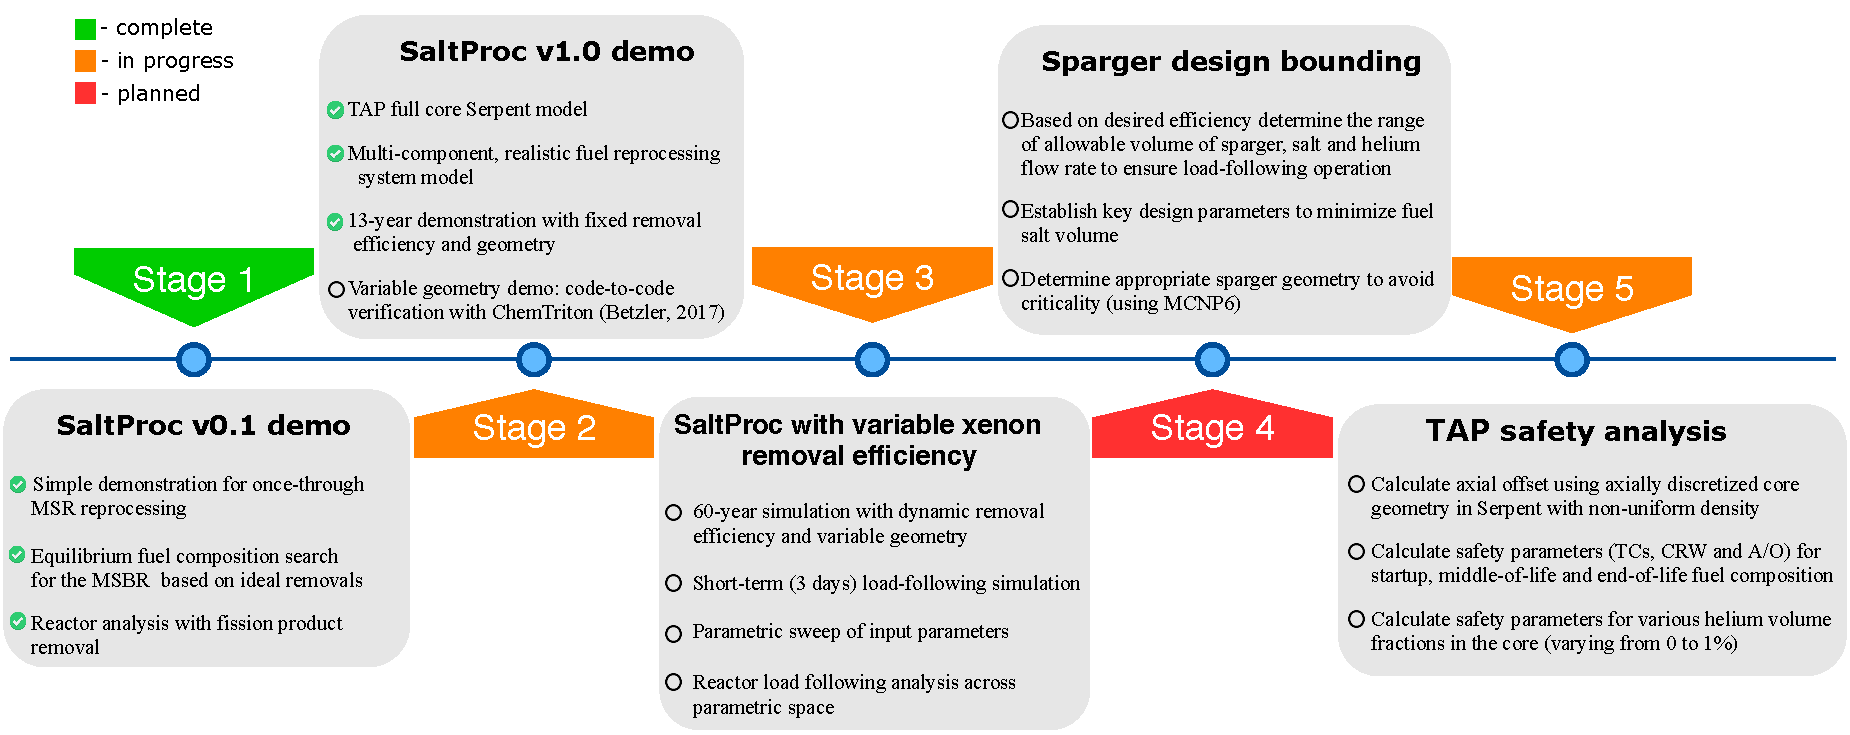
\includegraphics[width=\textwidth]{./images/progress_chart.pdf} 
	\caption{Workflow for the simulations proposed in this work.}
\end{figure}
		\end{textblock*}
\end{frame}


\subsection{Stage 1: Basic on-line reprocessing demonstration}

\begin{frame}
\frametitle{MSBR online reprocessing analysis}

\begin{columns}
	\column[t]{4.3cm}
	\begin{block}{SaltProc v0.1 demo for simple once-through \gls{MSR} 
	reprocessing}
		\fontsize{7}{9}\selectfont
		\begin{itemize}
			\item Full-core model of the \gls{MSBR} for 60 years of operation
			\item FP removal from the salt with fixed, ideal extraction 
			efficiencies 
			\item $^{233}$Pa ideal removal and feed of an equal mass of 
			$^{233}$U into the core
			\item Fresh fertile material feed to maintain the salt inventory
			\item Fine time resolution (3-day depletion steps)
		\end{itemize}
	\end{block}    	
	
	\column[t]{8cm}
		\begin{figure}[ht!] 
		\centering
			\includegraphics[width=\textwidth]{../figures/keff_msbr.png}
			\caption{Effective multiplication factor dynamics for the 
			full-core \gls{MSBR} model (reproduced from  
			Rykhlevskii \emph{et al.} \cite{rykhlevskii_modeling_2019}).}
		\end{figure}
	
\end{columns}
\end{frame}


\begin{frame}
\frametitle{Effect of fission products removal}       

\begin{figure}[t] % replace 't' with 'b' to force it to 
	\centering
	\includegraphics[width=0.8\textwidth]{../figures/keff_rem_cases.png} 
	\caption{Calculated effective multiplication factor for the full-core 
		\gls{MSBR} model with removal of various fission product groups over 
		10 	years of operation (reproduced from Rykhlevskii \emph{et al.} 
		\cite{rykhlevskii_modeling_2019}).}
\end{figure}

\end{frame}


\subsection{Stage 2: Tool demonstration and validation for \gls{TAP}}

\begin{frame}
\frametitle{\gls{TAP} concept high-fidelity Serpent model}
	  \begin{textblock*}{12.25cm}(0.25cm,1.8cm) % {block width} (coords)
\begin{figure}[htp!] % replace 't' with 'b' to 
	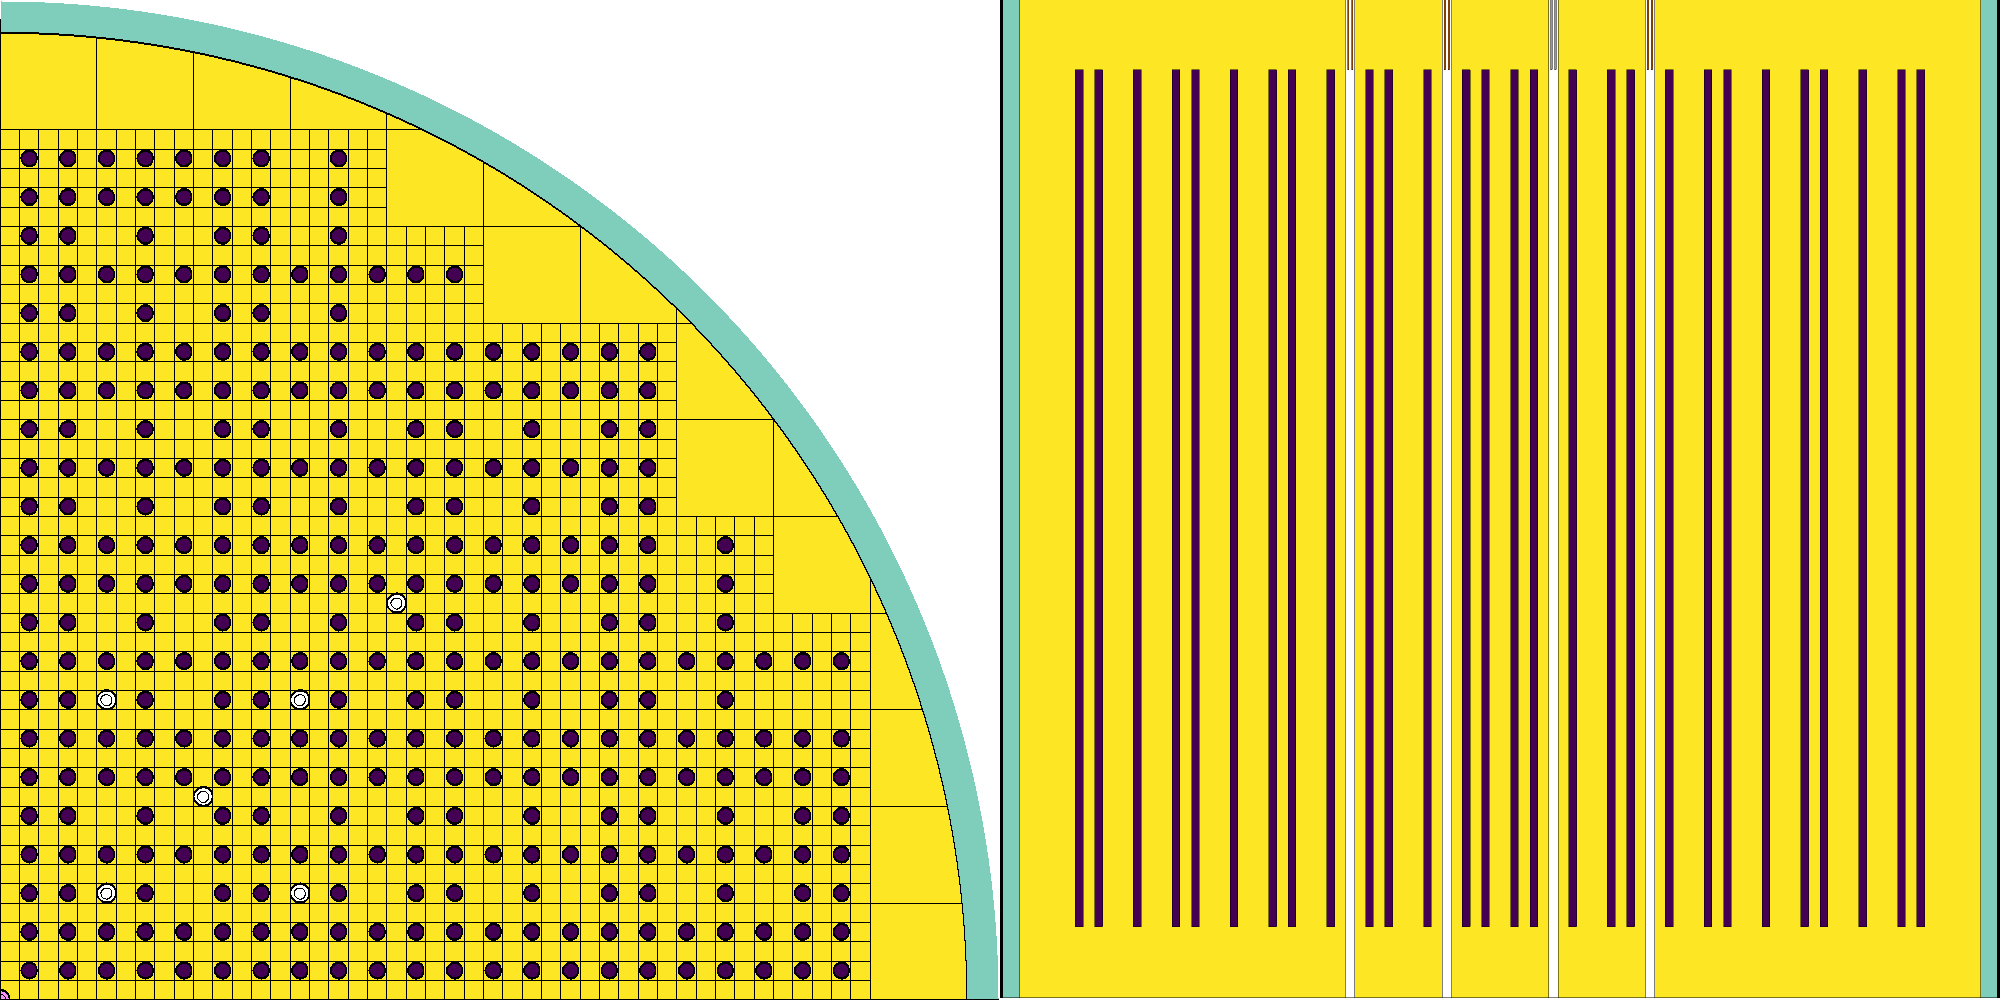
\includegraphics[width=\textwidth]{./images/tap_model.png}
	\caption{An $XY$ (left) and $XZ$ (right) section of the \gls{TAP} model. 
	The violet color represents
zirconium hydride, and the yellow represents 
	fuel salt 
	(reproduced from Rykhlevskii \& Huff \cite{rykhlevskii_milestone_2019}).}
\end{figure}
	  \end{textblock*}
\end{frame}


\begin{frame}
\frametitle{Multi-component fuel reprocessing system model in SaltProc}       

\begin{columns}
		\column[t]{6cm}
		\begin{itemize}
			\item Fixed, non-ideal ($<100\%$) removal efficiencies
			\item Sparger and separator located in-line
			\item Static geometry with constant moderator-to-fuel ratio
			\item 5\% and 19.79\% low-enriched uranium feed
		\end{itemize}

	\column[t]{6.5cm}
	\begin{figure}[htp!] % replace 't' with 'b' to 
	\centering
			\vspace{-7mm}
		\begin{overprint}
	\onslide<1>\includegraphics[height=0.8\textheight]{../figures/demo_reprocessing_scheme.png}
	\onslide<2>\includegraphics[height=0.8\textheight]{../figures/demo_reprocessing_scheme_2.png}
		\end{overprint}
	\caption{\gls{TAP} reprocessing scheme flowchart used for demonstration of 
		SaltProc \cite{rykhlevskii_milestone_2019}.}
	\end{figure}
\end{columns}
\end{frame}


\begin{frame}
\frametitle{Depletion simulation results for TAP with various feeds}       
\begin{textblock*}{12.6cm}(0.1cm,2.2cm) % {block width} (coords)
	\begin{figure}[htp!] % replace 't' with 'b' to 
		\begin{minipage}[b]{0.48\textwidth}
			\includegraphics[width=\linewidth]{../figures/keff_3.png}
		\end{minipage}
			\hspace{-2mm}
		\begin{minipage}[b]{0.48\textwidth}
			\includegraphics[width=\linewidth]{../figures/keff_zoomed_2.png}
		\end{minipage}
		\caption{Effective multiplication factor dynamics for full-core
		\gls{TAP} model for different fueling scenarios over a 13-year reactor 
		operation (left) and for the time interval from 367 to 471 days after 
		startup (right). Confidence interval $\pm\sigma=28pcm$ is shaded.}
	\end{figure}
\end{textblock*}
\end{frame}


\begin{frame}
\frametitle{Fuel salt composition evolution during the TAP operation}
\begin{textblock*}{12.25cm}(0.25cm,1.8cm) % {block width} (coords)
	\begin{figure}[htp!] % replace 't' with 'b' to 
		\centering
				\vspace{-3mm}
		\includegraphics[width=0.72\textwidth]{../figures/u_pu_mass.png}
		\caption{Mass of major nuclides during 13 years of reactor operation 
		with 19.79\% \gls{LEU} feed.}
	\end{figure}
\end{textblock*}
\end{frame}


\subsection{Stage 5: Safety parameters evolution}

\begin{frame}
\frametitle{Safety parameters calculations at start-up}       

\begin{columns}
	\column[t]{6cm}
	\begin{itemize}
		\item \gls{TAP} reactor operation range is 773-973K
		\item Temperature coefficient of reactivity calculated separately for 
		fuel and moderator in range 800-1000K
		\item Temperature coefficients are negative at start-up but are 
		expected to be more negative during operation
		\item A configuration of 25 control rods has a reactivity worth of 
		$1110\pm9.7$pcm (1.1\%) at startup
		\item Serpent template to calculate temperature coefficients and  
		control rod worth by single run was developed
	\end{itemize}
	
	\column[t]{6.5cm}
	\begin{figure}[bth!] % replace 't' with 'b' to 
	\includegraphics[width=\textwidth]{../figures/axial_offset.png}
	\caption{\gls{TAP} model divided to multiple axial layers with different 
	densities of the salt to calculate axial power offset.}
	\end{figure}
\end{columns}
\end{frame}

